\section{Experiments}

We assess the performance of the Base System on labyrinth environments. In all the experiments we consider, an agent is positioned in a starting location and it stochastically navigates the environment based on transition probabilities between states. For clarity, we split the experiments into two cases. The first is the case of timing, where $\sum = \{\sigma\}$ and the second is with multiple observations.

For timing, the goal is to make predictions about how long the agent will survive the environment. One can also ask conditional queries such as how long the agent should expect to survive given that t seconds have elapsed $f(\sigma^m|\sigma^n) = (eqns)$. 

For multiple observations we place the agent in the environment, let it transition between states for a fixed number of observations and then remove the agent. The goal for the multiple observation labyrinth will be to make predictions about seeing observation sequences. 

In both cases, we analyse the performance for M-PSRs of different model sizes with a fixed observation data set. For each Base System M-PSR, we set $\Sigma'$ to be {$\sigma^{2^k}, k<=256 $}. For the Data-Driven PSRs we learn 10 operators from the observations with the greedy learning algorithm for obtaining $\kappa$ described in (). For all the M-PSRs, we assign $\kappa$ to the dynamic programming algorithm given in (). 

To measure the performance of a PSR we use the following norm:
$||f - \hat{f}|| = \sqrt{\sum\nolimits_{x \in observations}(f(x) - \hat{f(x)})^2}$. We use this norm because of a bound presented by [AUTHORS], which states that (). Here the function f denotes the true probability distribution over observations and the function $\hat{f}$ denotes the function associated with the learned M-PSR/PSR. In the environments that we consider the function f is obtainable directly as we have access to the underlying HMMs.

Since the set of observations $\Sigma^*$ is infinite, we compute approximations to this error norm, by fixing a set of strings T and summing over T. For the timing case, we take T to be the $\{sigma^k, k<=n\}$, while for the multiple observation case, we take all possible strings producible from the prefixes and suffixes in our dataset. That is, for the multiple observation case $T = \{p \cdot c, \forall p \in P, s \in S\}$.

\subsection{Learning PSRs for Timing}
For the timing case, we construct our empirical hankel matrix by including ${\sigma^i i<=n}$. With this choice, the empirical hankel matrix will be a nxn matrix with the prefixes and suffixes being the same.The parameter n depends on the application. For Double Loop environments we set n to be 300, while for pacman n was set to 600. The important property that needs to be satisfied when choosing the parameter n is that enough observations are captured to learn a good model. Something here: $\lim_{ \to 2} f(x) = 5$ .

\subsection{Learning PSRs for Multiple Observations}

For multiple observations a slightly more complex approach is required to construct the empirical hankel matrix. For prefixes, we select the k most frequent prefixes from our observations set. For suffixes we take all suffixes that occur from our set of prefixes. We also require prefix completeness. That is if $p is a prefix of p', then p is also included$ This heuristic for constructing empirical hankel matrices was given in previous work by [] and it showed that ().

\subsection{Double Loop Timing}

For timing, we start by considering a double loop environment. The lengths of the loops correspond to the number of states in the loop. Figure 1 shows the results of a 64-16 double loop, while Figure 2 shows the results for a 47-27 double loop. Here the lengths correspond to the number of states there are in each loop. In our environments, one time step corresponds to one state transition. A trajectory begins with the agent starting at the intersection of the two loops. At the intersection, the agent has a 50 percent chance of entering either loop. At intermediate states in the loops the agent moves to the next state in the loop with probability p and remains in its current state (it self-transitions) with probability 1-p. Exit states are located halfway between each loop. At an exit state, the agent has a 50 percent probability of exiting the environment. For Double Loop environments we learn the PSRs and M-PSRs with 10 different datasets of 10000 observation sequences. For a fixed dataset, we compare the performance of a PSR and different M-PSRs and then plot the average error over the 10 datasets.

\begin{figure}[ht!]
\centering
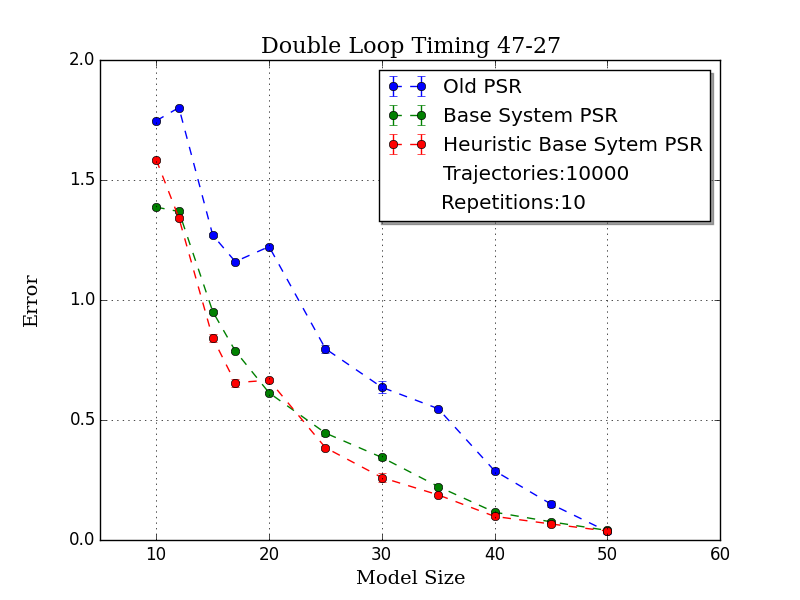
\includegraphics[width=60mm]{uCOREPICS/DoubleLoopTimingHeuristics47-27.png}
\caption{Double Loop Environment\label{overflow}}
\end{figure}

\begin{figure}[ht!]
\centering
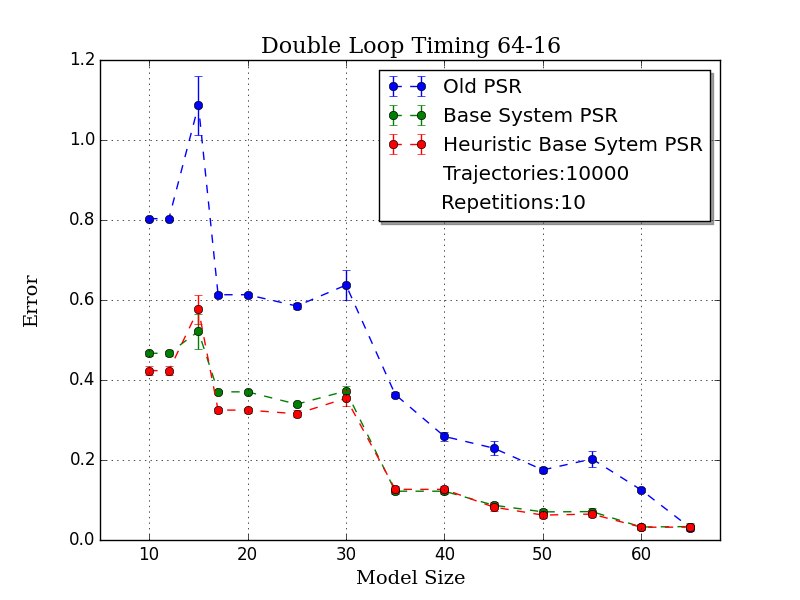
\includegraphics[width=60mm]{uCOREPICS/DoubleLoop64-16Heuristics.png}
\caption{Double Loop Environment\label{overflow}}
\end{figure}

\subsection{Pacman Timing}

As M-PSRs seemed to have strong benefits Double-Loop environments, we moved on to a more complex system: Pacman. The Pacman labyrinth's graphical representation is shown in figure (). The figure shows the transition structure and edge weights. Edge weights vary from 1 to 3 and are stretched by a parameter which we call the stretch factor SF. We set SF at 10, but similar results hold for other settings. As with Double-Loops we use 10 datasets of 10000 observations plot the average error for the learned PSRs and different types of M-PSRs.

\begin{figure}[ht!]
\centering
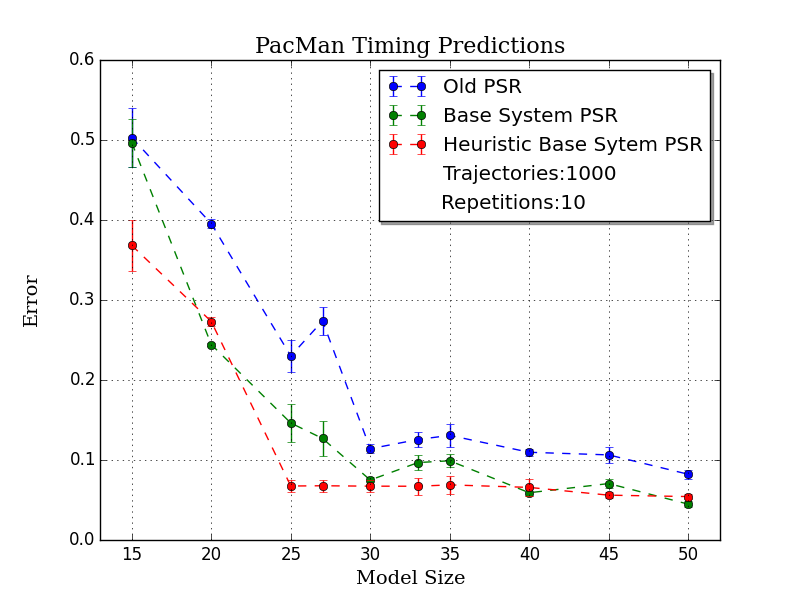
\includegraphics[width=60mm]{uCOREPICS/PacManTimingHeuristicsIncluded.png}
\caption{Double Loop Environment\label{overflow}}
\end{figure}

\begin{figure}[ht!]
\centering
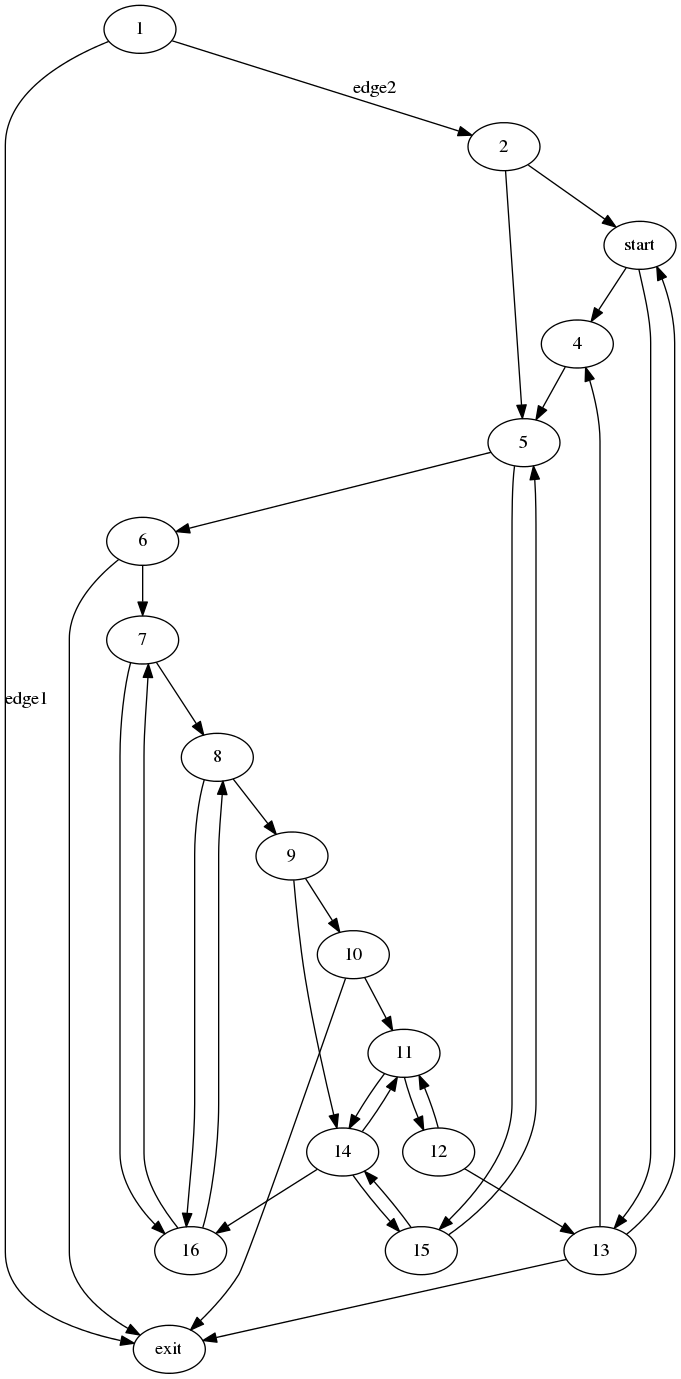
\includegraphics[width=60mm]{uCOREPICS/graphPacMan.png}
\caption{Double Loop Environment\label{overflow}}
\end{figure}

\subsection{Timing - Results}
For Timing, M-PSRs all perform perform significantly better than the standard PSR for reduced model sizes. As the model size gets close to the  number of states learned by the model. For lower datasizes ... In addition, the heuristic based approach performs slightly better than the powers of two method. For the double loop case the heuristic approach learns multiples of the loop lengths which results in partitions which use fewer operators. As an example, for the 47-27 labyrinth the heuristic included included the following operators: $\Sigma'=\{\sigma^47, sigma^27 ...\}$ For Pacman, the operators that are learned are various multiples of the stretch factor, which once again shows that the greedy heuristic is effective. The top 7 of 10 operators are usually learned consistently, while the other strings vary slightly dependent on the dataset of 10000 trajectories.

\subsection{Multiple Observations}

We now move to the multiple observation case. Here the Data-Driven M-PSRs really show their strength as observation sequences are more complex. We construct a Double Loop environment where one loop is green and the other is blue. The lengths of each loop are also varied, see Figure 4 and Figure 5. We fix the length of observations to be $loop1 + loop2 * 3$. To build empirical estimates of probabilities we set f(x)=prefix-occ(x)/num-strings-length>=x. This means that the PSRs will compute the probability of a prefix occuring.

\subsection{Multiple Observations Results}

\begin{figure}[ht!]
\centering
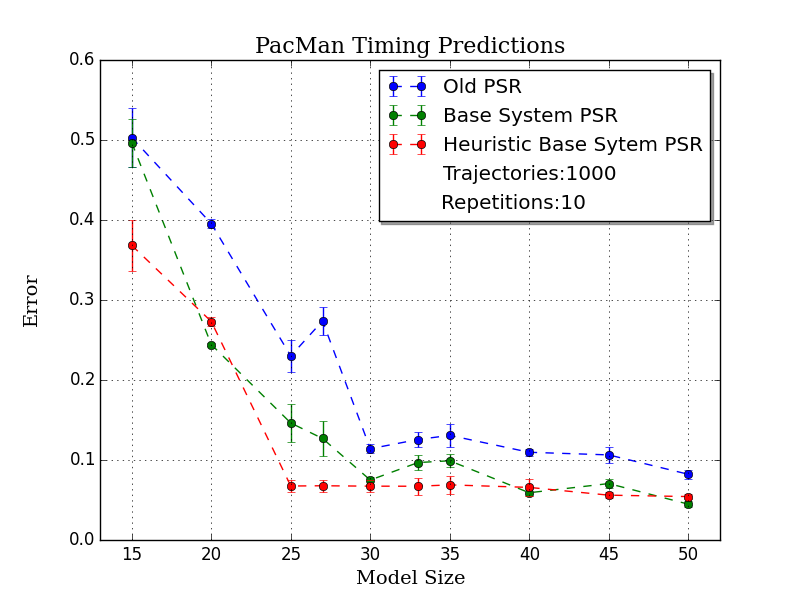
\includegraphics[width=60mm]{uCOREPICS/PacManTimingHeuristicsIncluded.png}
\caption{Double Loop Environment\label{overflow}}
\end{figure}
